\section{Impact on Network Design}
\label{sec:network_design}

\begin{figure*}
\vspace{2mm}
\centering
    \subfigure[Max Timeliness vs. Network Size (Sum Sim. = 5.0)]{
	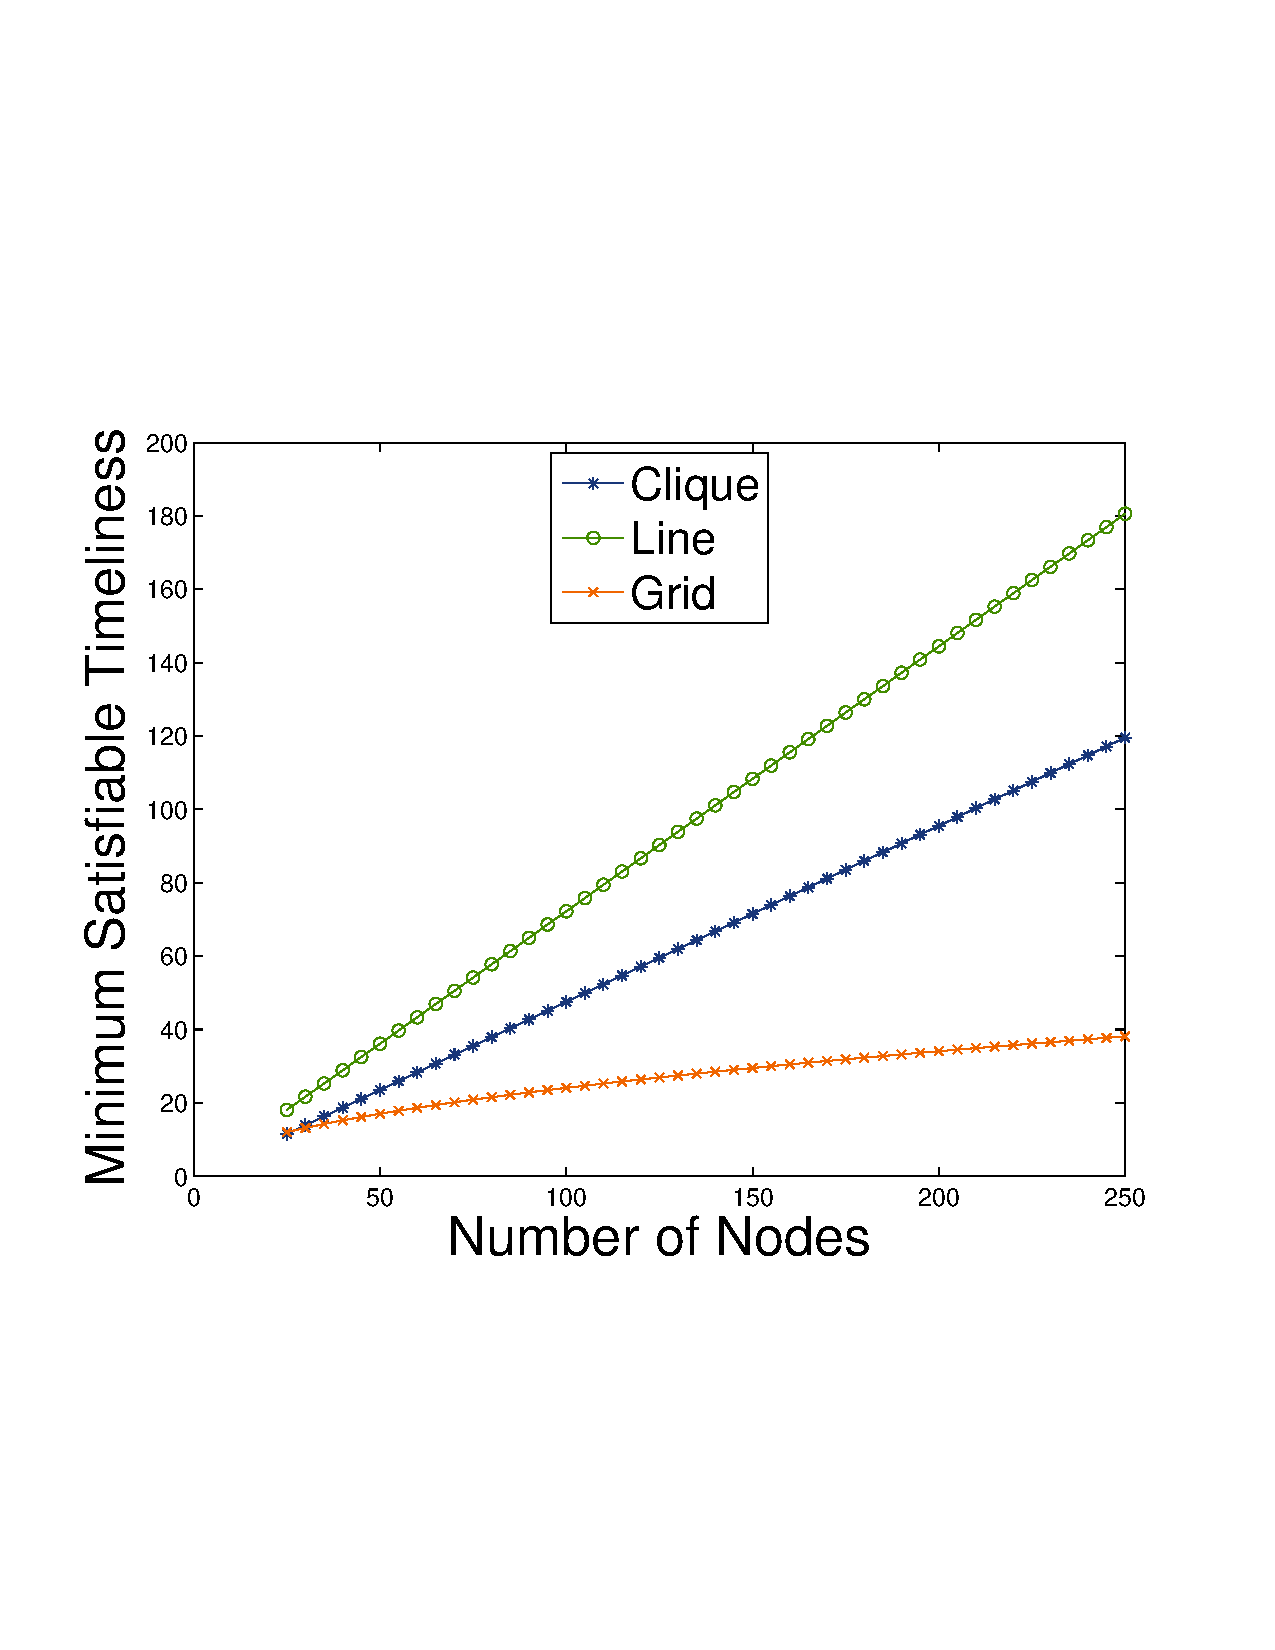
\includegraphics[scale=0.22, clip=true, trim=14mm 65mm 25mm 65mm]{figures/use_cases_examples/tness_vs_num_nodes_5_SS_12_IS_2_W_color.pdf}
        \label{fig:use_case_tness_vs_num_nodes}
        }
    \subfigure[Max Sum Sim. vs. Network Size (Timeliness = 50)]{
	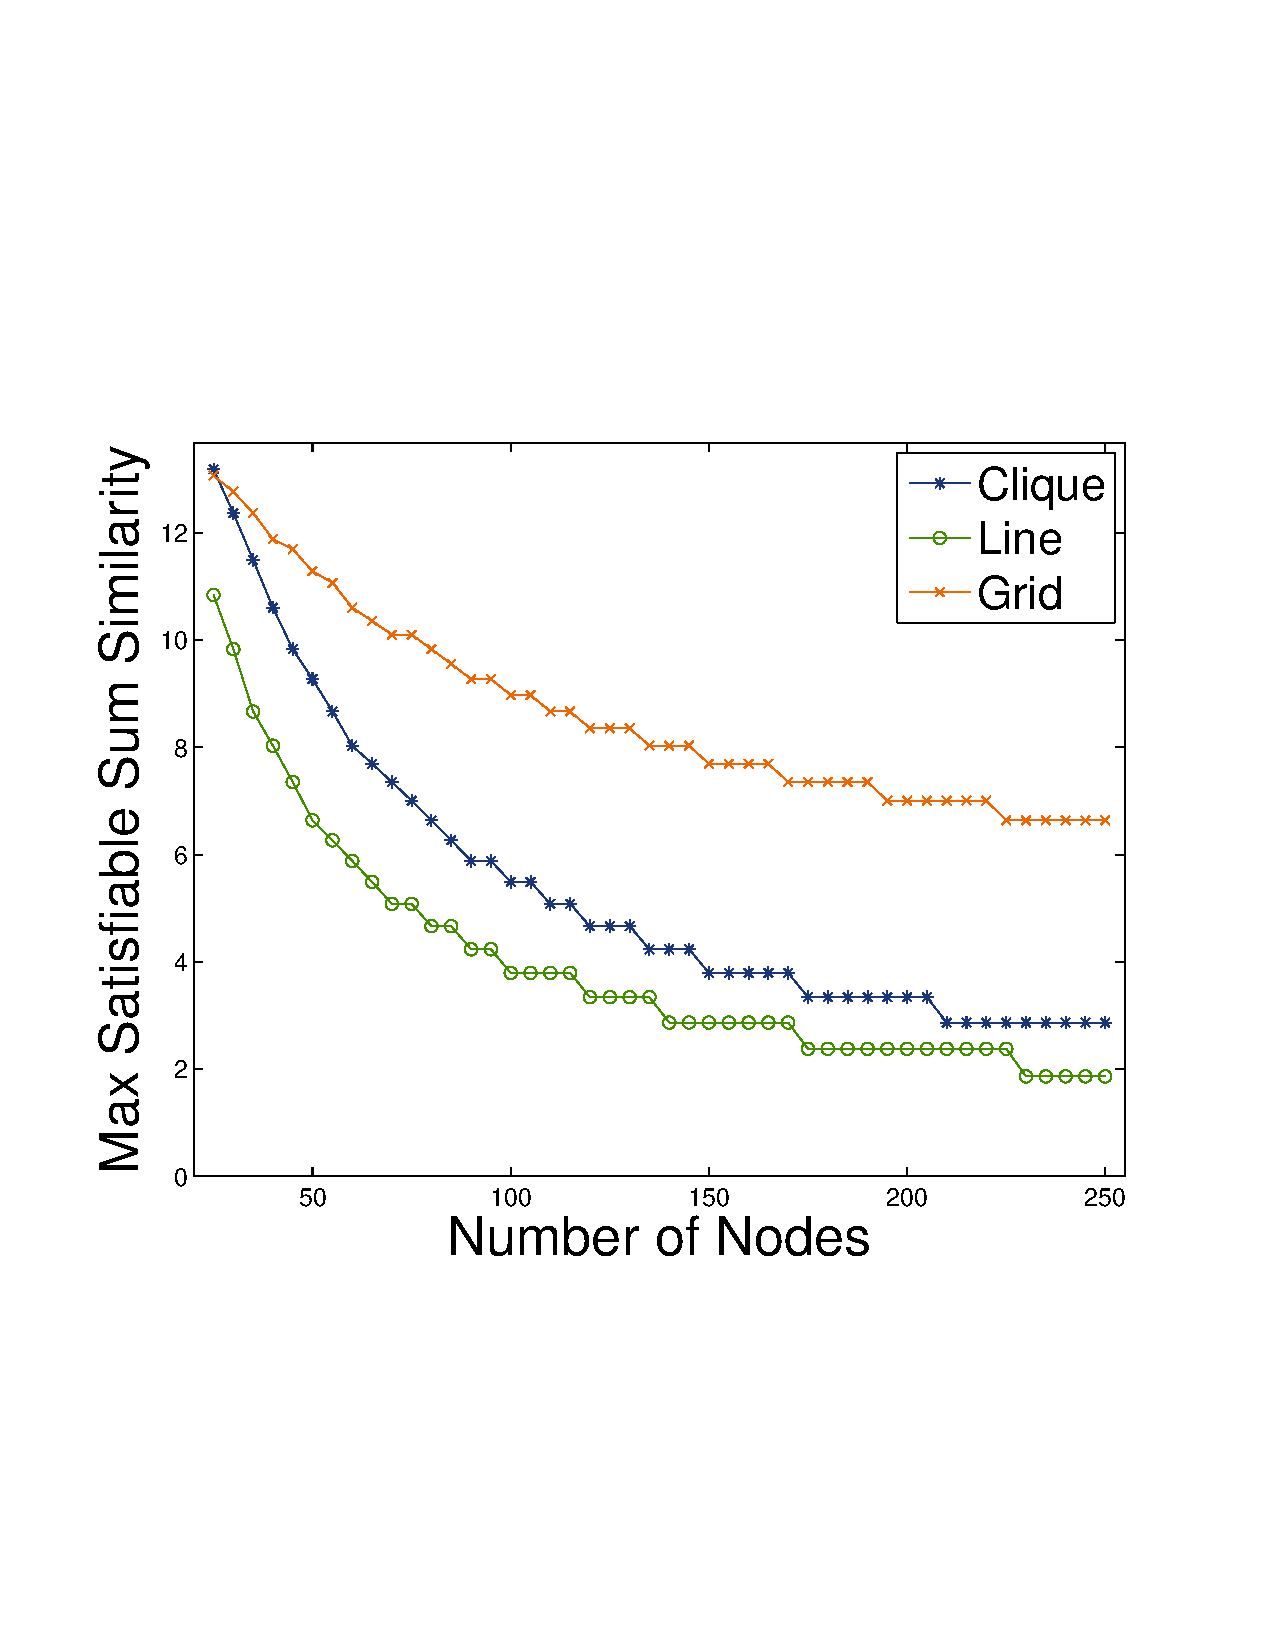
\includegraphics[scale=0.22, clip=true, trim=14mm 65mm 25mm 65mm]{figures/use_cases_examples/sum_sim_vs_num_nodes_50_T_12_IS_2_W_color.pdf}
        \label{fig:use_case_sum_sim_vs_num_nodes}
        }
  \subfigure[Max Network Size vs. Sum Sim. (Timeliness = 10)]{
	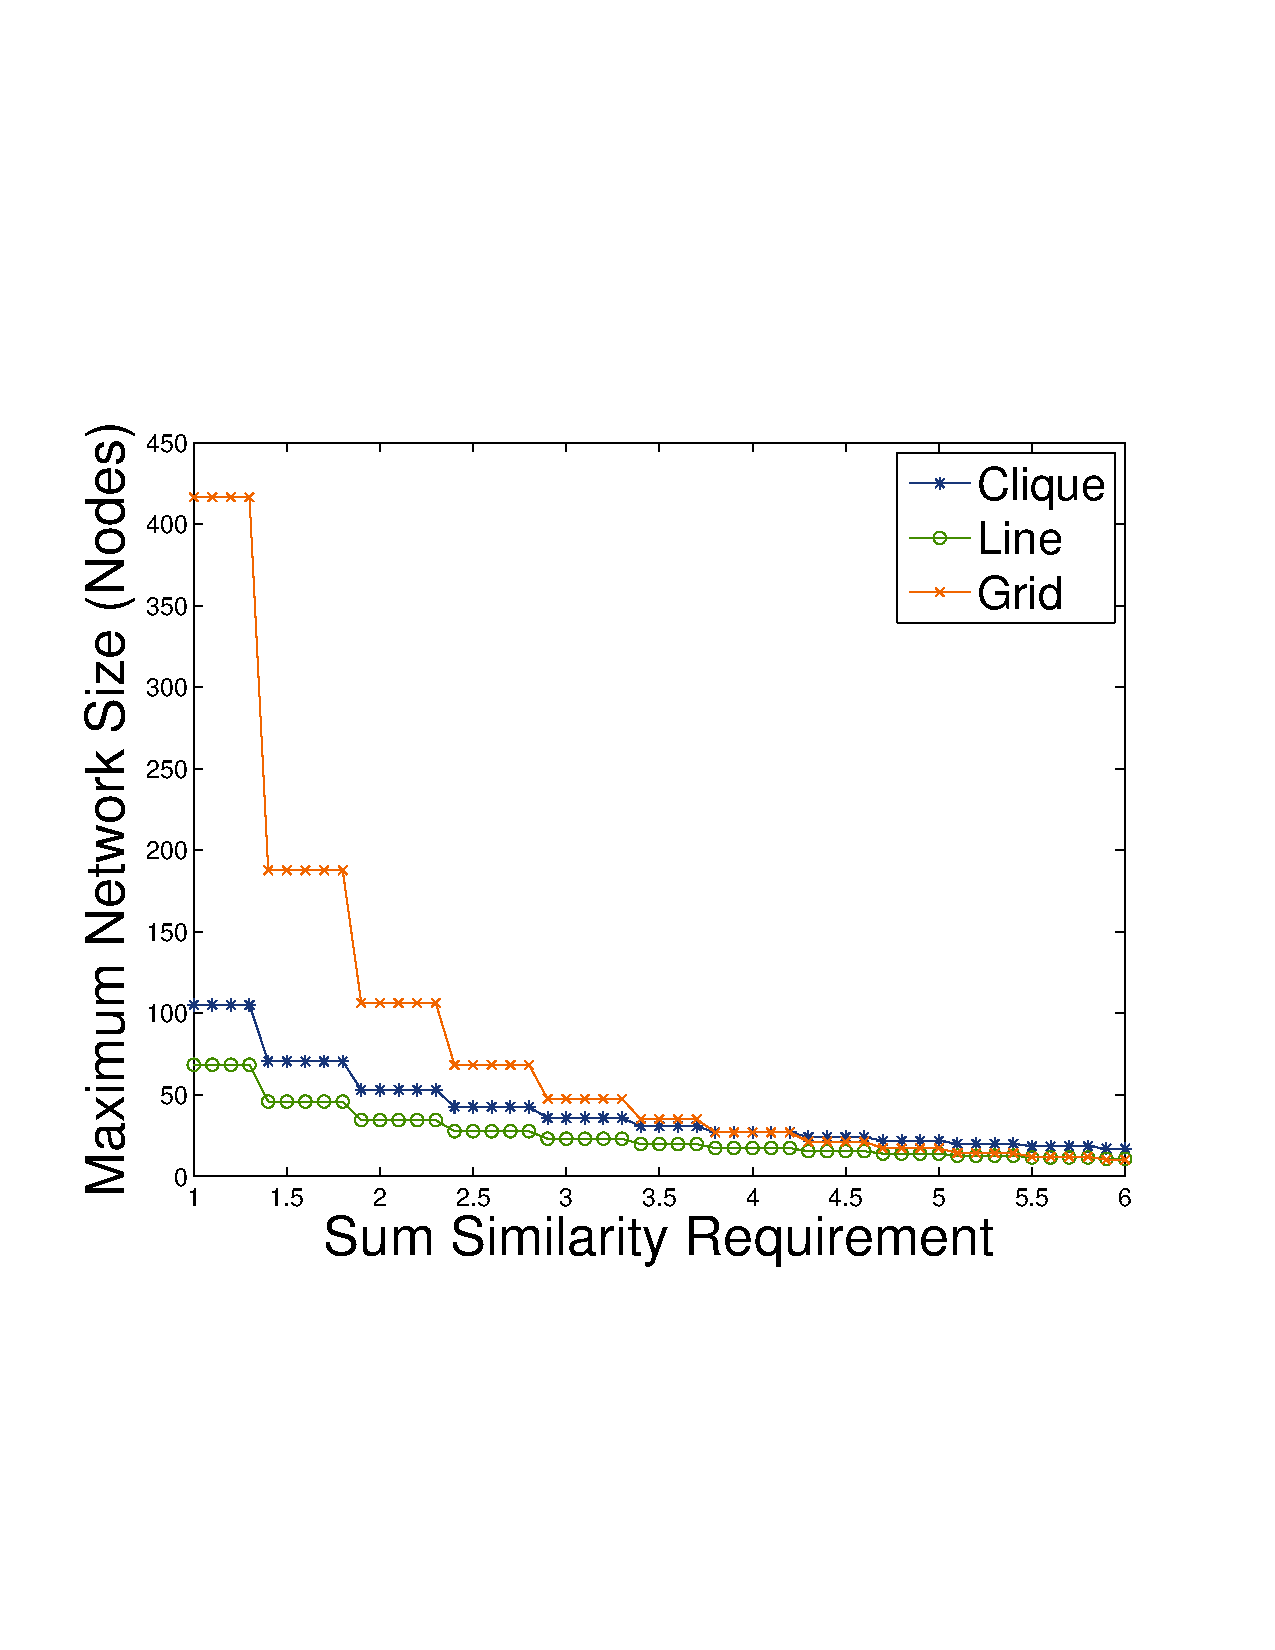
\includegraphics[scale=0.22, clip=true, trim=14mm 65mm 25mm 65mm]{figures/use_cases_examples/num_nodes_vs_sum_sim_10_T_12_IS_color.pdf}
        \label{fig:use_case_num_nodes_vs_qoi}
        }
  \subfigure[Max Network Size vs. Timeliness (Sum Sim. = 5.0)]{
	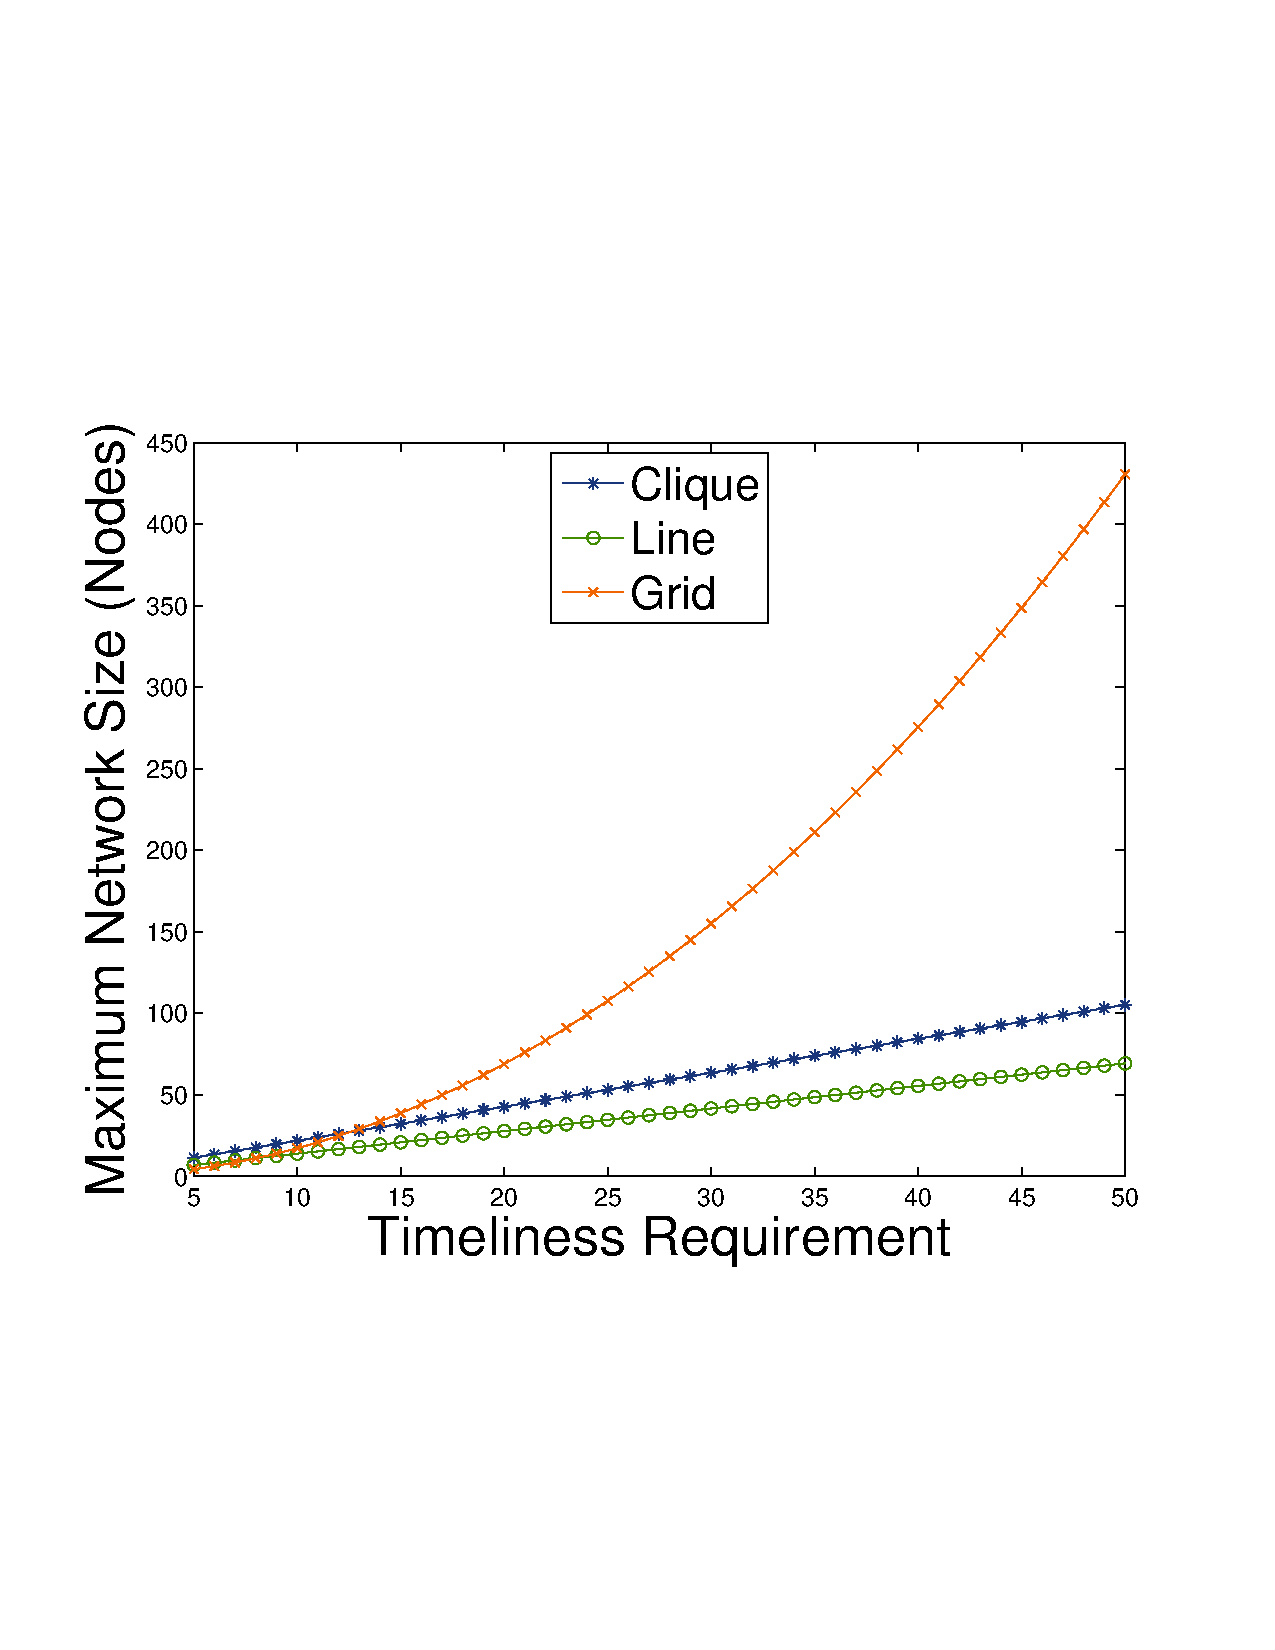
\includegraphics[scale=0.22, clip=true, trim=14mm 65mm 25mm 65mm]{figures/use_cases_examples/num_nodes_vs_tness_5_SS_12_IS_color.pdf}
        \label{fig:use_case_num_nodes_vs_qoi_2}
        }
   \vspace{-1mm}
   \caption{Varying design parameters provide immediate limitations as well as evident trends and comparisons.}
   \label{fig:huh_net_design}
   \vspace{-6mm}
\end{figure*}
 
Now that we have established a model for QoI satisfiability and scalability and shown its accuracy in predicting estimated limits, we show how it can also provide quick, but useful intuition about the impact of various network parameters.  Once an equation for a network's limitations is formulated as was done for equations in Table \ref{table:scal_eqs} %(\ref{eq:clique_gen})-(\ref{eq:grid_gen})
, it can be solved for a single parameter to gain an understanding of its reliance on the other factors.  This analysis can be done very quickly and easily by approximating when appropriate, or by using symbolic and/or numerical solvers.  To exemplify this application in network design, we have applied this process to the equations in Table \ref{table:scal_eqs} % (\ref{eq:clique_gen})-(\ref{eq:grid_gen}) 
and created several figures that provide insight into network limitations and tradeoffs.

Figure \ref{fig:use_case_tness_vs_num_nodes} shows minimum satisfiable timeliness values for different topologies of increasing size.  While it may be intuitive that a grid network should be able to serve flows with lower timeliness constraints than a line network since it will have shorter average path lengths, what is not intuitive is \emph{how much} lower of a timeliness constraint is satisfiable.  Here, we see that a grid network can scale up to over $250$ nodes while supporting flows with $T = 40$.  A line network, on the other hand, can only scale to only approximately $20\%$ of that network size for the same timeliness value.  %In either case, it is intuitive to know how a clique network's timeliness satisfiability should respond to either a grid or line network since its operation is quite different.

Figure \ref{fig:use_case_sum_sim_vs_num_nodes} visualizes sum similarity limits for network instances with timeliness fixed.  Here, again, limits and trends are quickly evident.  In addition, the nonlinearity of completeness requirements are manifested here as the data requirements for the highest completeness requirements are only sustainable for small networks, but as the network size increases, the impact on achievable completeness is not as dramatic.  

%To highlight this example, we can refer back to Figure \ref{fig:topkAvgNumSameSet} and see that in order to obtain $7$ images matching the target image on average, we should collect $~28$ images, which we see from \ref{fig:topkSumSim} equates to a sum similarity of approximately $6.5$.  If we require a timeliness of $50$ seconds and our network topology has $50$ nodes that are in a line, a sum similarity of $6.5$ is the maximum completeness the network can support.  If these same nodes are arranged in a grid network, however, we see that the network still has the capability to support more traffic, closer to a sum similarity of $11.5$, which is twice as many images on average.

Finally, given a topology and application with predetermined requirements of $\mathbf{q}$, we may be simply interested in how large our network can grow before its capacity to deliver the desired QoI is no longer possible.  Values that answer this question are in Figures \ref{fig:use_case_num_nodes_vs_qoi} and \ref{fig:use_case_num_nodes_vs_qoi_2}.  Once again, the graphs show the major impact completeness and timeliness requirements can have on network size.  Figure \ref{fig:use_case_num_nodes_vs_qoi} especially shows the impact of using completeness instead of simply throughput as the non-linear relationship of completeness to data rate pointed out in Section \ref{sec:qoi_model} is evident here.

%In this section, we approximate where appropriate like in (\ref{eq:tness_line_1})-(\ref{eq:tness_line}) below since the insights we seek here are more easily gained with simpler expressions, and are not greatly affected for large values.  In applying the framework in practice, though, numerical solvers can be used, removing the need for approximation.    

%Throughout this section, channel rate and packet size values are again fixed at $W = 2$ Mbps and $P_S = 1,500$ Bytes.  Also, we again choose sum similarity as the illustrative metric of completeness, but any other definition of completeness could be swapped in here.  Specific values of $SS$, $T$, and $N$ are varied to show various effects, so their values are explicitly listed in each figure and/or description.

%\subsubsection{Timeliness}
%Since $\mathbf{q}$ is a composite requirement of both timeliness and sum similarity, the value representing completeness in this application, we can explore the limits and impact of network parameters on each separately.  First, we will substitute appropriate values for each topology, and then solve the inequality for $T$. The result for each is as follows:
%
%\vspace{4mm}
%\noindent
%Clique:
%\begin{equation}
%	T \geq \frac{B}{W} \cdot (N -1) + \frac{P_S}{W}
%\label{eq:tness_clique}
%\end{equation}
%Line:
%\begin{eqnarray}
%\label{eq:tness_line_1}
%	T &\geq& 1.5 \cdot \frac{B}{W} \cdot \frac{(N-1)^2}{N-2} + 1.5 \cdot \frac{P_S}{W} \cdot (\frac{N}{4} - 1) \\
%	&\approx& 1.5 \cdot \frac{B}{W} \cdot (N-1) + 1.5 \cdot \frac{P_S}{W} \cdot (\frac{N}{4} - 1)
%\label{eq:tness_line}
%\end{eqnarray}
%Grid:
%\begin{equation}
%	T \geq 5 \cdot \frac{\sqrt{N}}{W} \cdot (B + \frac{P_S}{3})
%\label{eq:tness_grid}
%\end{equation}

%Using these inequalities, not only can network designers gain estimates of maximum timeliness constraints satisfiable in various network scenarios, but they can also quickly compare the dependency on specific parameters.  By quick examination of these relationships, one can see that timeliness has a $O(N)$ relationship with respect to network size in clique and line topologies, but $O(\sqrt{N})$ in a grid topology.  Figure \ref{fig:use_case_tness_vs_num_nodes} reinforces this lesson.  The graph shows minimum $T$ values for increasing values of $N$ with all other values fixed, showing that a grid network can serve tighter timeliness constraints than other topologies in larger networks.

%While it may have been intuitive that a grid network should be able to serve flows with lower timeliness constraints than a line network since it will have shorter average path lengths, what is not intuitive is \emph{how much} lower of a timeliness constraint is satisfiable.  For example, we see here that a grid network can scale up to over $250$ nodes while supporting flows with $T = 40$.  A line network, on the other hand, can only scale to only approximately $20\%$ of that network size for the same timeliness value.  In either case, it is intuitive to know how a clique network's timeliness satisfiability should respond to either a grid or line network since its operation is quite different.  With the inequalities in (\ref{eq:tness_clique})-(\ref{eq:tness_grid}), though, it is quickly and easily understood.

%\begin{figure}[ht]
%\centering
%\subfigure[Achievable Timeliness vs. Network Size for a fixed Sum Similarity = 5.0]{
%	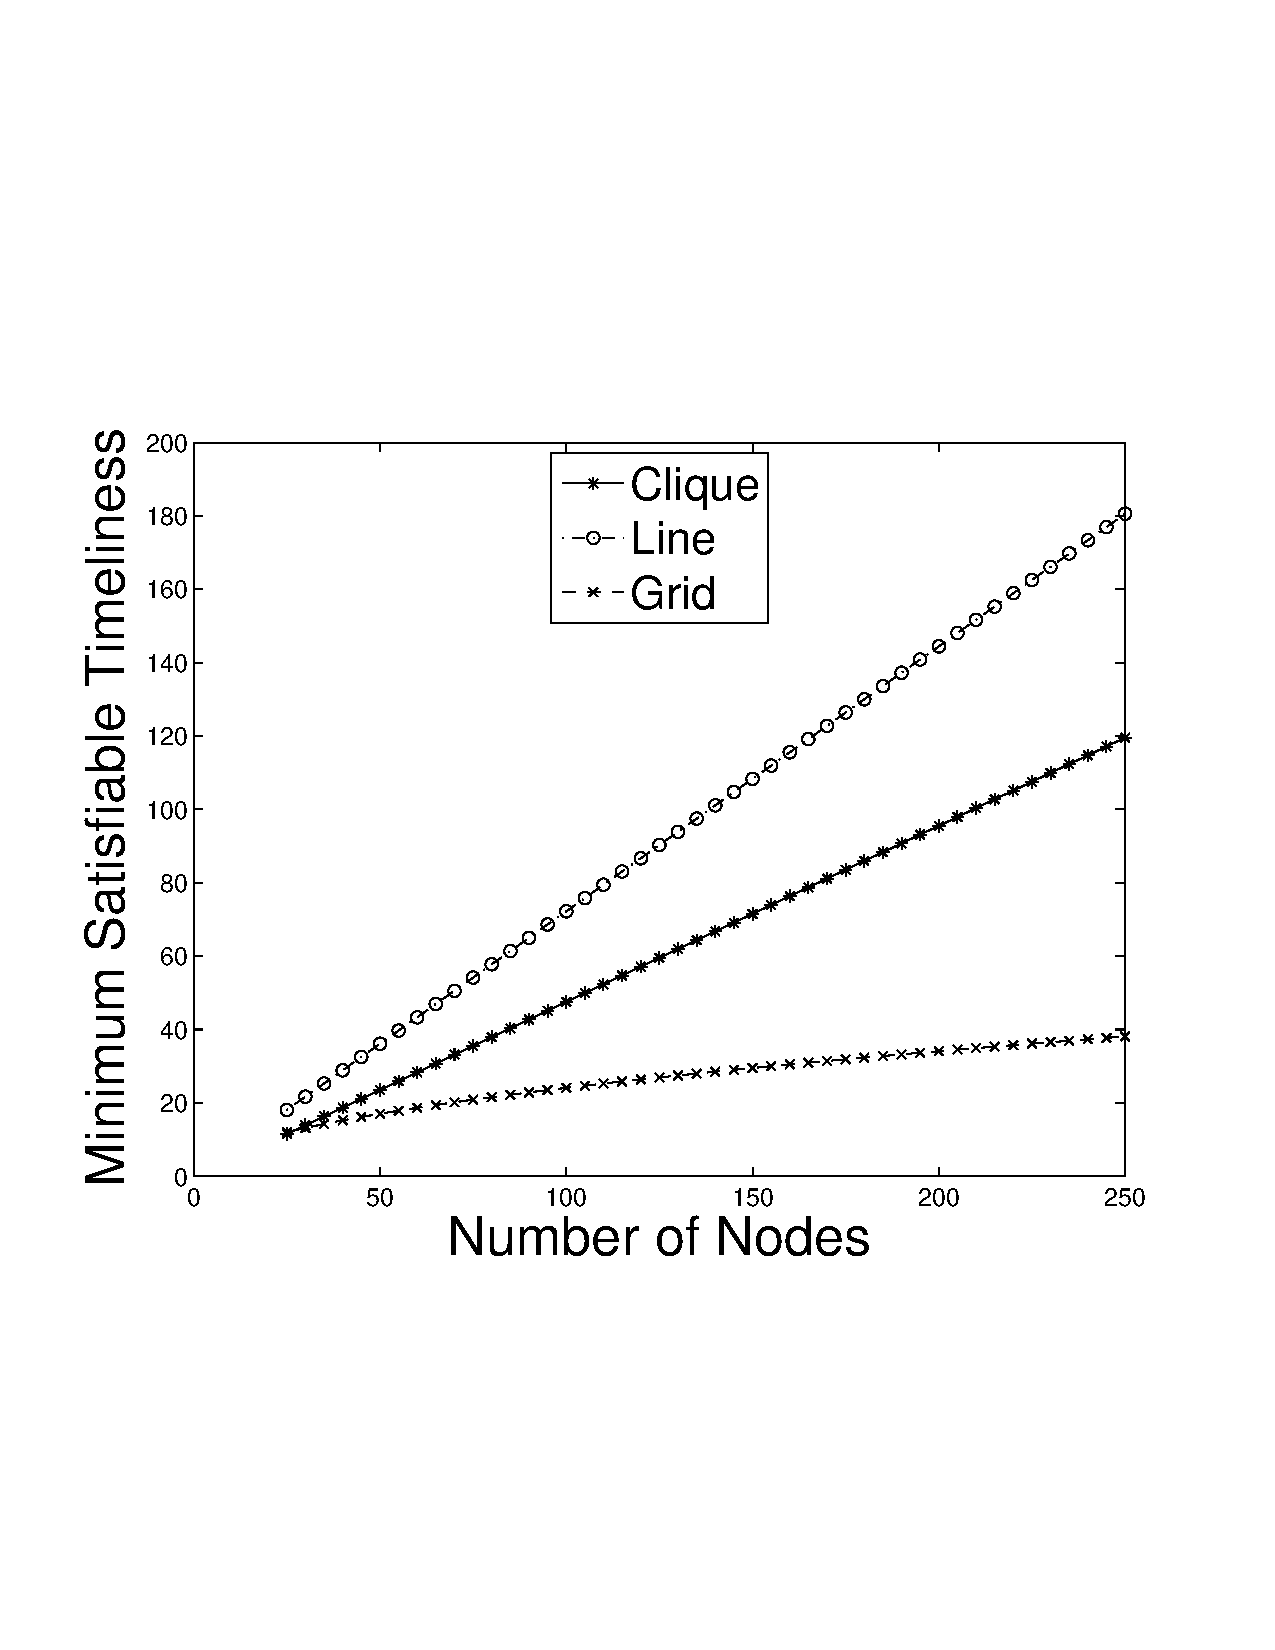
\includegraphics[scale=0.31, clip=true, trim=15mm 65mm 20mm 65mm]{figures/use_cases_examples/tness_vs_num_nodes_5_SS_12_IS_2_W.pdf}
% 	\label{fig:use_case_tness_vs_num_nodes}
%	}
%\subfigure[Achievable Sum Similarity vs. Network Size for a fixed Timeliness = 50]{
%	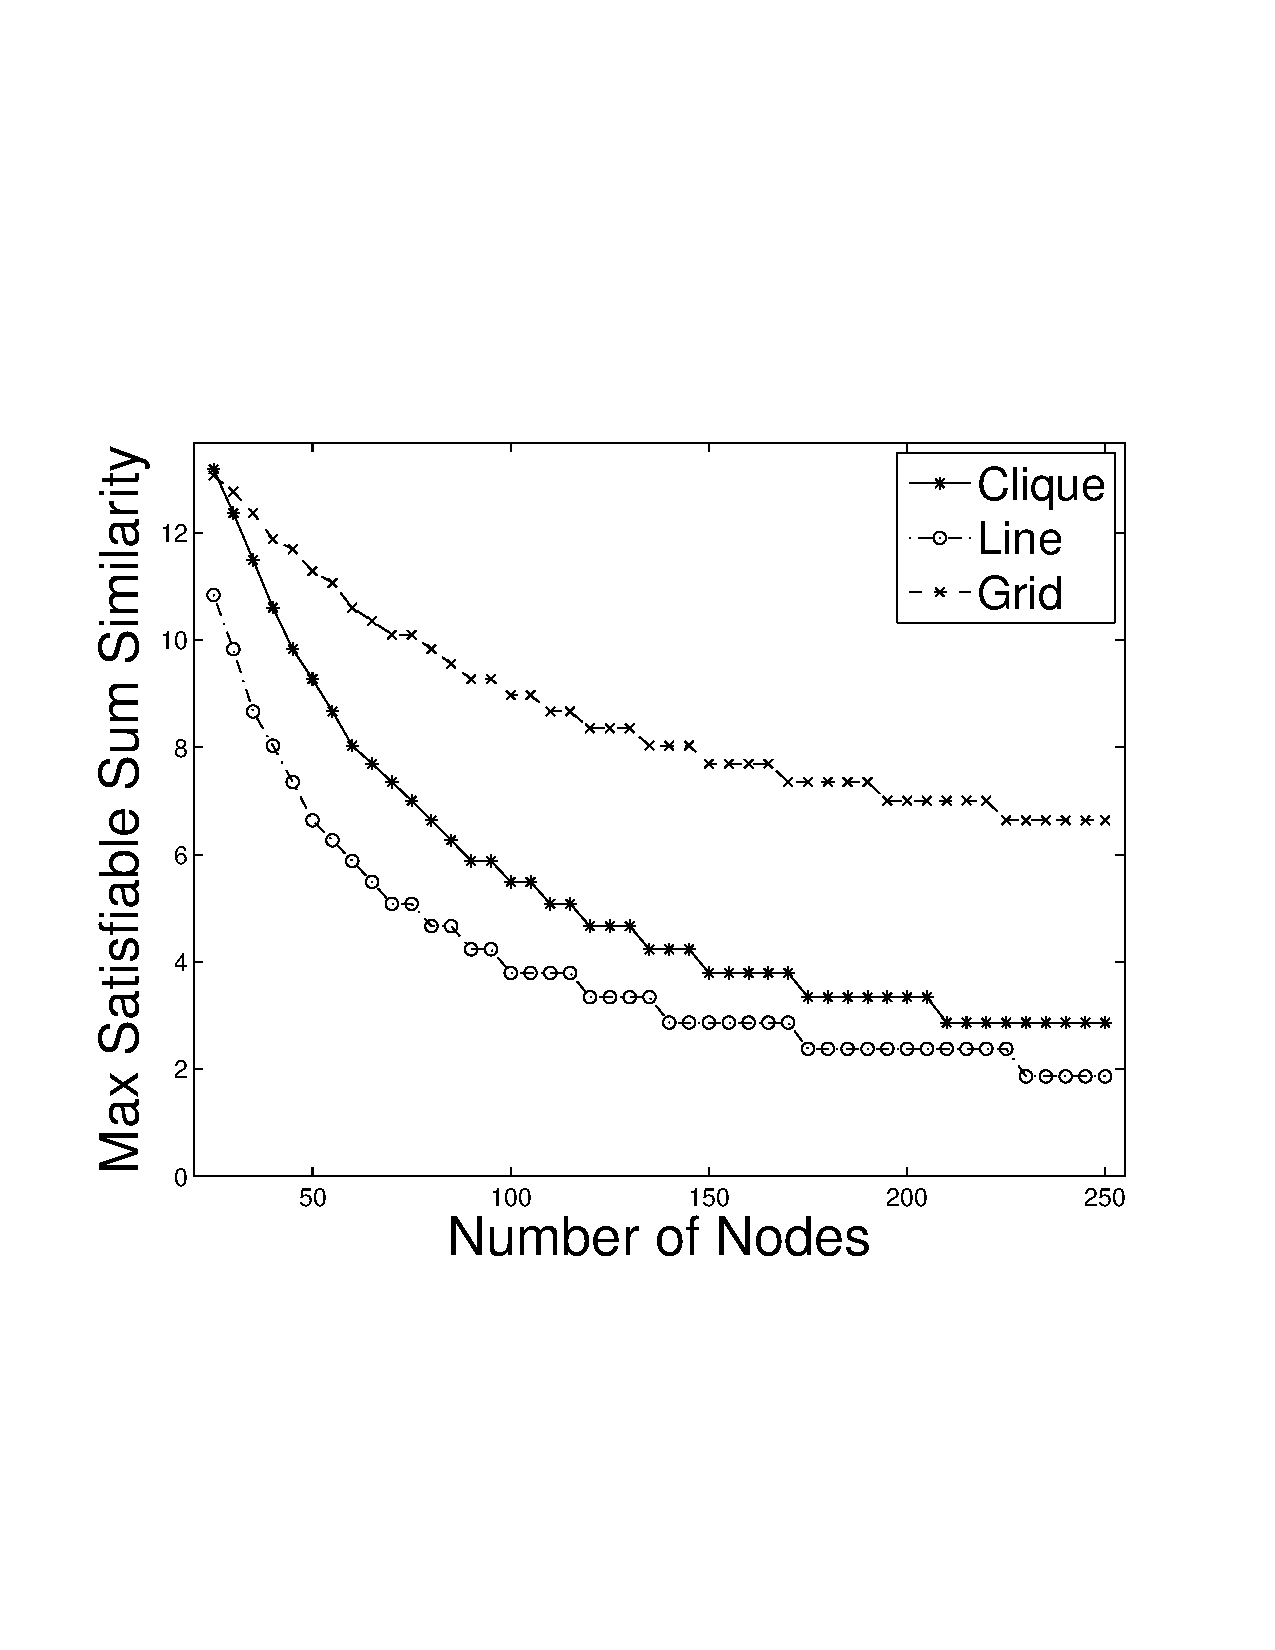
\includegraphics[scale=0.31, clip=true, trim=15mm 65mm 20mm 65mm]{figures/use_cases_examples/sum_sim_vs_num_nodes_50_T_12_IS_2_W.pdf}
%	\label{fig:use_case_sum_sim_vs_num_nodes}
%	}
%\caption{Achievable QoI values are quickly evident for various network sizes and comparisons between topologies are easily made.}
%\vspace{-2mm}
%\end{figure}
%
%\begin{figure}[ht]
%\centering
%  \subfigure[Varying Sum Similarity (T = 10)]{
%	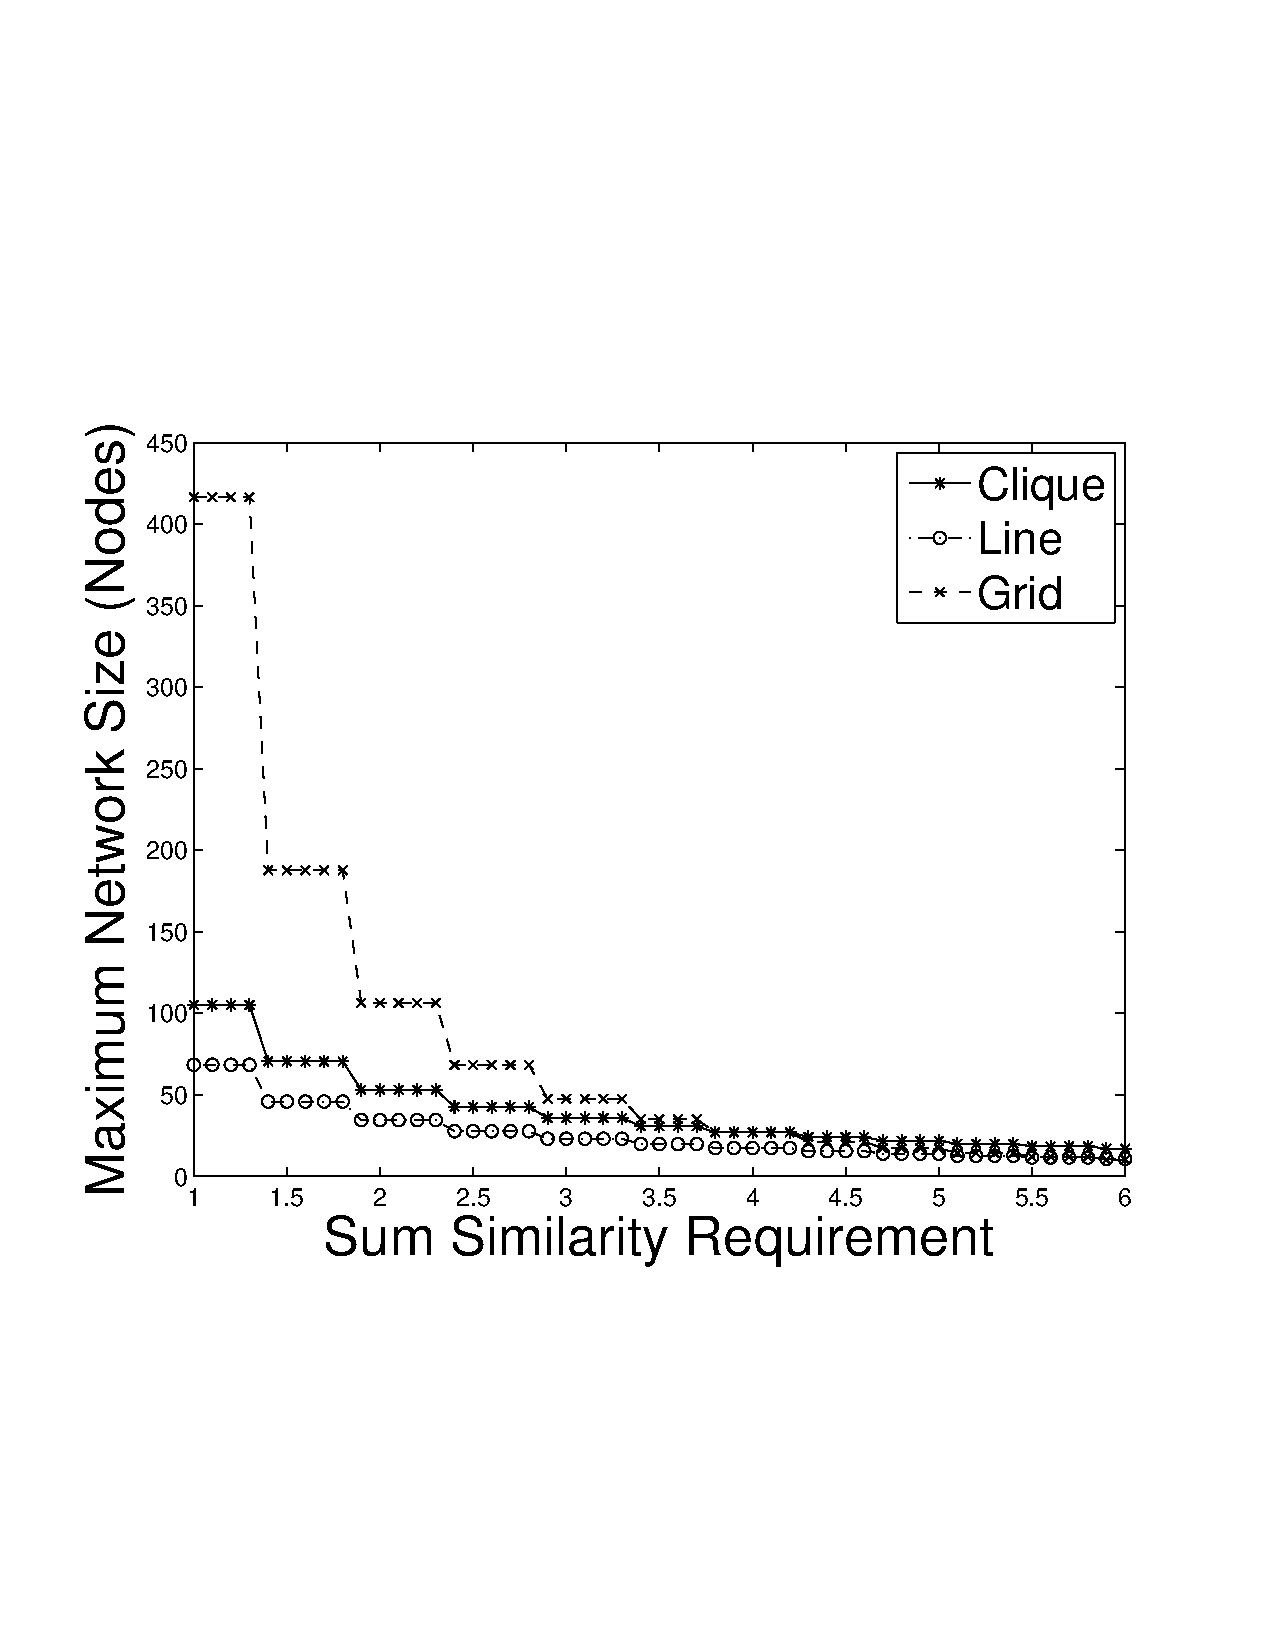
\includegraphics[scale=0.31, clip=true, trim=15mm 65mm 20mm 65mm]{figures/use_cases_examples/num_nodes_vs_sum_sim_10_T_12_IS.pdf}
%	}
%  \subfigure[Varying Timeliness (SS = 5.0)]{
%	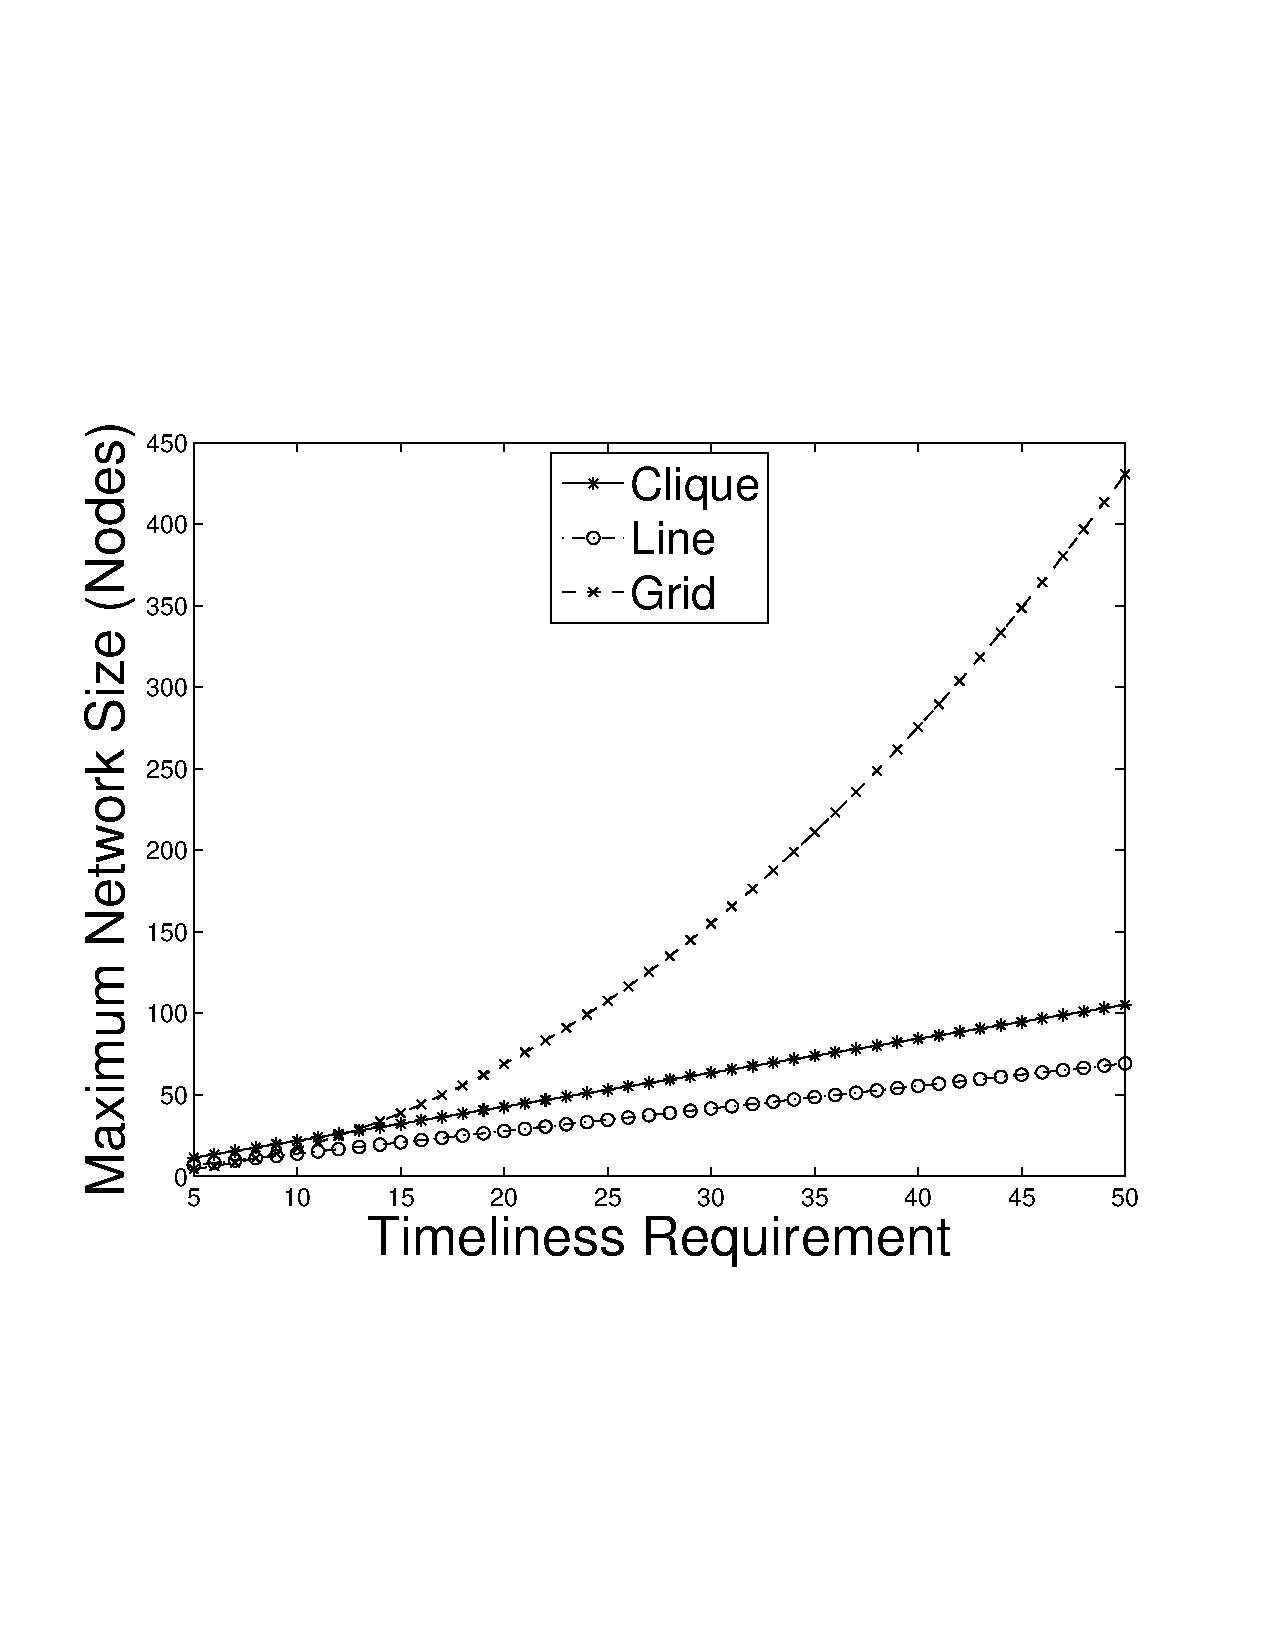
\includegraphics[scale=0.31, clip=true, trim=15mm 65mm 20mm 65mm]{figures/use_cases_examples/num_nodes_vs_tness_5_SS_12_IS.pdf}
%	}
%\caption{Achievable Network Size for Varying QoI Requirements}
% \label{fig:use_case_num_nodes_vs_qoi}
%    \vspace{-7mm}
%\end{figure}

%\subsubsection{Sum Similarity (Completeness)}
%
%In the exact same manner, we can evaluate maximum sum similarity values, $SS$, achievable by a network.  To do so, we define the inverse of the function $Q(SS) = k_{req}$ defined above.  Here, $Q'(k_{req}) = SS$ provides the sum similarity corresponding to the number of images served in each flow.  The relationship for sum similarity for each topology is described with the following relations:
%
%\vspace{4mm}
%\noindent
%Clique:
%\begin{equation}
%	SS \leq Q'( \frac{W \cdot T - P_S}{I_s \cdot (N-1)} )
%\end{equation}
%Line:
%\begin{equation}
%	SS \leq Q'( \frac{W \cdot T - 1.5 \cdot P_S \cdot (\frac{N}{4} - 1)}{3 \cdot I_s \cdot \frac{(N-1)^2}{2(N-2)}} )
%\end{equation}
%Grid:
%\begin{equation}
%	SS \leq Q'( \frac{W \cdot T - 2.5 \cdot P_S \cdot (\frac{2}{3} \cdot \sqrt{N} - 1)}{5 \cdot I_s \cdot \sqrt{N}} )
%\end{equation}
%
%Figure \ref{fig:use_case_sum_sim_vs_num_nodes} visualizes these sum similarity limits for network instances of different numbers of nodes while timeliness is fixed.  Here, again, limits and trends are quickly evident.  In addition, the nonlinearity of completeness requirements are manifested here as the data requirements for the highest completeness requirements are only sustainable for small networks, but as the network size increases, the impact on achievable completeness is not as dramatic.  
%
%To highlight this example, we can refer back to Figure \ref{fig:topkAvgNumSameSet} and see that in order to obtain $7$ images matching the target image on average, we should collect $~28$ images, which we see from \ref{fig:topkSumSim} equates to a sum similarity of approximately $6.5$.  If we require a timeliness of $50$ seconds and our network topology has $50$ nodes that are in a line, a sum similarity of $6.5$ is the maximum completeness the network can support.  If these same nodes are arranged in a grid network, however, we see that the network still has the capability to support more traffic, closer to a sum similarity of $11.5$, which is twice as many images on average.
% 
%\subsubsection{Scalability}
%
%Finally, given a topology and application with predetermined requirements of $\mathbf{q}$, we may be simply interested in how large our network can grow before its capacity to deliver the desired QoI is no longer possible.  The proper relationships to answer this question are below in (\ref{eq:scal_clique})-(\ref{eq:scal_grid}), and Figure \ref{fig:use_case_num_nodes_vs_qoi} gives maximum scalability examples when either component of $\mathbf{q}$ is varied.  Once again, the graphs show the major impact completeness and timeliness requirements can have on network size.
%
%\vspace{4mm}
%\noindent
%Clique:
%\begin{equation}
%	N \leq \frac{W \cdot T - P_S}{B} -1
%\label{eq:scal_clique}
%\end{equation}
%Line:
%%\begin{equation}
%%	W \cdot T - 3 \cdot B \cdot \frac{(N-1)^2}{2(N-2)} - 1.5 \cdot P_S \cdot (\frac{N}{4} - 1)
%%\end{equation}
%%\indent which can be approximated to:
%\begin{equation}
%	N \leq \frac{W \cdot T + \frac{3}{2}P_S}{\frac{3}{2}B+\frac{3}{8}P_S}
%\label{eq:scal_line}
%\end{equation}
%Grid:
%\begin{equation}
%	N \leq (\frac{W \cdot T}{5 \cdot B + \frac{5}{3} \cdot P_S})^2
%\label{eq:scal_grid}
%\end{equation}


